% \section*{Introduction}
Human computer interaction has been evolving over the past decades. With development in technologies, the physical contact between the computer and the human is decreasing rapidly. Advanced systems which work on speech and gesture control still require a minimal effort from the user to interact with the machine. Though these effort seem to be mere, it is a challenging task for humans with disabilities. Systems which work on facial gestures bridge this gap to an extent but it does not completely decode the actual intent of the person. Brain Computer Interface paves way to encode the persons intent and thoughts without the need for any physical effort. It provides enormous capabilities for physically challenged people to express themselves just by their thoughts. 

Autonomous vehicles are the future of mobility, several companies around the world invest and research on new technologies to solve new challenges that appear in developing level 5 autonomy. The level of human interaction with the vehicle has been decreasing with increasing safety. However including humans in the loop is necessary at certain times to avoid any undesirable events. Level 5 autonomous vehicles is still a long way to go, but by bringing in a minimal interaction of the driver with the system, safety can be improved. One of the ways of achieving it is interfacing the thought and decision process of the driver to the autonomous vehicle, a process commonly referred to as Brain-Computer-Interface (BCI)\nomenclature{BCI}{Brain-Computer-Interface}. 

Once shown in science fiction novels and movies, Brain-Computer Interface (BCI) has become widely researched and developed in the academic institutions and industries in the past decades. It has been applied and tested on mammals for a wide range of applications. However it has its own challenges and limitations. With evolving technologies, new innovations and discoveries, BCI systems are built to understand and decode the brain waves better. The analysis of the brain signals have seen a shift in the paradigm with the introduction of machine learning techniques. 

Modern BCI design involves understanding brain dynamics, pattern recognition in the brain waves, deriving relevant features from the measured brain waves. However it is very challenging to create a BCI system that can work on any person, as the brain signals are task-specific and brain signal signatures are very unique to a person. The cortex folding and the relevant functional maps are different across individuals. Even for the very same person, the brain dynamics are non-stationary at all time scales. In addition, it is almost impossible to place the electrodes exactly on the same location for every recording sessions. Further the psychological states of the user such as boredom, distraction and similar factors play a significant role in the quality of the signal measured. The Signal-to-Noise Ratio (SNR) \nomenclature{SNR}{Signal-to-Noise Ratio} in a brain signal is very poor, making it difficult to obtain required information from brain signals. It is harder to spatially measure the data from one region as large collections of neurons are involved in many different activity, not just one. These challenges can vary a lot depending on the methods used to record and analyse the brain signals as well as the task that needs to be achieved. 

Given the challenges, the goal of this work is to steer a simulated car in the CARLA environment using brain signals obtained from the OpenBCI headgear. CARLA is an open-source simulator to develop, train and validate autonomous driving systems. OpenBCI is an open-source BCI platform that develops hardware and software for BCI scientific research. The brain signal from a 16 channel OpenBCI headgear is fed through a signal processing pipeline to extract the relevant Motor Imagery (MI) \nomenclature{MI}{Motor Imagery}features and classify the users intention. The signal preprocessing pipeline constitutes reliable and conventional signal processing techniques as well as state-of-the-art deep learning techniques. Several tools, libraries and frameworks such as MNE, Numpy, Scipy, Scikit-learn and PyTorch are used to achieve the goal. The communication between the OpenBCI system and the signal processing pipeline is established using Lab Streaming Layer (LSL)\nomenclature{LSL}{Lab Streaming Layer}. The signal processing pipeline classifies the signal into left, right or straight steering command and it is sent to CARLA through Robotic Operating System (ROS 1) framework\nomenclature{ROS 1}{Robotic Operating System-1}. The algorithms are packed into a ROS package which consists of multi-threaded nodes enabling real-time information transfer to CARLA. All the relevant code and references are made available in GitHub\cite{BCI_MotionControl}. Several open-source datasets are used to setup the basic brain signal processing pipeline and later tuned to work with the data obtained form the OpenBCI headgear.

\section{Environment setup}
The specifications of the system used for this project are listed in the table \ref{tb:specs}. The overview of the implemented system is given in the figure \ref{fig:MT_Overall}.

\begin{figure}[H] 
    \begin{center}
    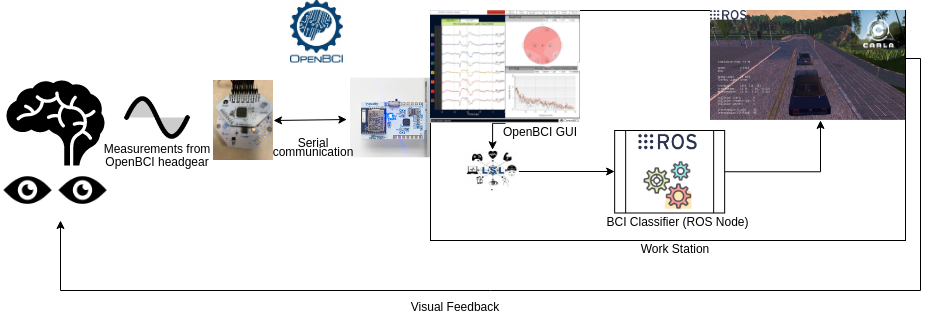
\includegraphics[width=1.0\textwidth]{images/MT_Overall.png}
    \caption{System overview}
    \label{fig:MT_Overall}
\end{center}
\end{figure}

\begin{table}[h!]
\centering
\arrayrulecolor[rgb]{0.8,0.8,0.8}
\begin{tabular}{|l|l|} 
\arrayrulecolor{black}\hline
\multicolumn{2}{|c!{\color{black}\vrule}}{Hardware Specifications}                                                                 \\ 
\hline
Processor                                   & AMD® Ryzen 7 4800h with radeon graphics × 16                                         \\ 
\arrayrulecolor[rgb]{0.8,0.8,0.8}\hline
RAM                                         & 16GB                                                                                 \\ 
\hline
Operating System                            & Ubuntu 20.04.5 LTS 64-bit                                                            \\ 
\hline
\# CPU cores                                & 8                                                                                    \\ 
\hline
GPU                                         & NVIDIA GeForce RTX 2060/ \\ 
                                            & RENOIR (renoir, LLVM 14.0.5, DRM 3.42, 5.15.0-56-generic)  \\ 
\hline
Graphic Card Driver                         & 515.86.01                                                                            \\ 
\hline
CUDA                                        & 11.6                                                                                 \\ 
\hline
cuDNN                                       & 8.3.2                                                                                \\ 
\hline
Cython + Daisy                              & 3.0.0                                                                                \\ 
\hline\\
\hline
%\multicolumn{1}{|l!{\color{black}\vrule}}{} & \multicolumn{1}{l!{\color{black}\vrule}}{}                                           \\ 
\arrayrulecolor{black}\hline
\multicolumn{2}{|c!{\color{black}\vrule}}{Software Specifications}                                                                 \\ 
\hline
Visual Studio Code                          & 1.74.0                                                                               \\ 
\arrayrulecolor[rgb]{0.8,0.8,0.8}\hline
OpenGUI                                     & 5.1.0                                                                                \\ 
\hline
CARLA                                       & 0.9.11 (py3.7-linux-x86\_64)                                                         \\ 
\hline\\
\hline
%\multicolumn{1}{|l!{\color{black}\vrule}}{} & \multicolumn{1}{l!{\color{black}\vrule}}{}                                           \\ 
\arrayrulecolor{black}\hline
\multicolumn{2}{|c!{\color{black}\vrule}}{Libraries and Frameworks}                                                                \\ 
\hline
Numpy                                       & 1.22.3                                                                               \\ 
\arrayrulecolor[rgb]{0.8,0.8,0.8}\hline
Pytorch                                     & 1.12.0+cu116                                                                         \\ 
\hline
MNE                                         & 1.2.0                                                                                \\ 
\hline
OpenCV                                      & 3.4.15                                                                               \\ 
\hline
scipy                                       & 1.8.1                                                                                \\ 
\hline
sklearn                                     & 1.1.1                                                                                \\ 
\hline
matplotlib                                  & 3.4.2                                                                                \\ 
\hline
kymatio                                     & 0.2.1                                                                                \\ 
\hline
PIL                                         & 7.0.0                                                                                \\ 
\hline
pandas                                      & 1.1.4                                                                                \\ 
\hline
Optuna                                      & 3.0.0                                                                                \\
\hline
\end{tabular}
\caption{\label{tb:specs} System and software specifications used for this project.}
\arrayrulecolor{black}
\end{table}

\section{Outline} 
The thesis is organized as follows the chapter \ref{ch:background} provides insight on different brain signal recording techniques, various EEG paradigms, brain signal extraction methods, artifact removal techniques used in this work and brief description of feature extraction, selection and classification steps, \ref{ch:sp_bci} discusses on various feature extraction and classification techniques used in brain signal analysis, \ref{ch:DL_bci} discusses on different SOTA Deep Learning techniques used in BCI signal analysis that can work as feature extractor and classifier. In chapter \ref{ch:cmp_bnch}, the tools and libraries used in this work are explained. The implemented algorithms are compared and analysed for different combinations. Finally chapter \ref{ch:ch_cncl} discusses about the challenges faced, further enhancements and the systems applicability for different use cases.

The following chapters provide deeper intuition and understanding of the methods researched and used in accomplishing this work. Finally the chosen algorithm is used to steer the simulated car in CARLA through ROS.